\documentclass[11pt,a4paper]{article}
\usepackage{setspace}
\usepackage{amsmath}
\usepackage{amsfonts}
\usepackage{graphicx}
\usepackage[margin=0.75in,top=0.75in,bottom=0.75in]{geometry}
\usepackage{hyperref}
\usepackage{helvet}
\renewcommand{\familydefault}{\sfdefault}
% \usepackage{subfloat}
% \usepackage{fancyhdr}

\graphicspath{ {.} }
% \pagestyle{fancy}
% \fancyfoot{}
% \pagestyle{empty}

\title{\vspace{-1.4cm}\Large Positron Emission Tomography Image Reconstruction Algorithms}
\date{}
\author{Zong Fan \\Email: \href{mailto:zongfan2@illinois.edu}{zongfan2@illinois.edu}}

\begin{document}
    \maketitle
    \vspace{-1.2cm}
    \section{Introduction}
    Positron Emission Tomography (PET) is a functional imaging technique by injecting radioactive substances called radiotracer into a patient's body and then measuring the distribution of the radioisotopes, which reflects the changes in metabolic or other physiological processes. The concept of emission tomography was introduced by David E. Kuhl in the late 1950s and was further developed by Gordon Brownell and William Sweet to build the first PET scanner at 1972\cite{portnow2013history}. Since that, due to its ability to image tissue activities in vivo and to detect low-concentration radiotracer sensitively and quantitatively, PET has been widely employed in various clinical applications, such as disease diagnosis, monitoring progression of disease and treatment response in oncology, glucose metabolism measurement in live tissue, blood flow measurement in the brain. 

    PET projection data cannot be directly interpreted by observers, and reconstruction into images is required. The reconstruction of the radiotracers' distribution mapping function is solved as an inverse problem. However, it's crucial to limit the radiation dose on patients from the injected radiotracer. Dose reduction usually suffers elevated noise level, which would largely cause the mapping function ill-posed. In order to reduce the impact of high-level noise on imaging quality and to improve spatial resolution, various researches have been devoted to optimizing the reconstruction methods\cite{tong2010petctreview}, which is the field we would discuss in the following text. Section \ref{sec:principle} describes the imaging principle of PET. Section \ref{sec:method} introduces commonly-used reconstruction methods and their shortcomings. Finally, Section \ref{sec:future} focuses on the future development of reconstruction methods and the challenges.

    \vspace{-0.5cm}
    \section{Reconstruction Principle}
    \label{sec:principle}
    \textbf{Photon detection to projection data:} The brief principle of data acquisition for imaging is described here. First, radiotracer, a functional compound (e.g. glucose) labeled with short half-life positron-emitting radioisotope (e.g. fluorine-18), is injected into the patient. After a waiting period when the radiotracer accumulates in the tissues of interest where it is metabolized, the patient is placed in the scanner. As the radioisotope decays to a stable state, the emitted positron travels a short distance in the tissue (typically $<1mm$) and interacts with an electron, a process called annihilation that produces a pair of 511keV annihilation photons moving in approximately opposite directions. When reaching the detector, they create a burst of light detected by photomultiplier tubes in the scanner. If the two photons are detected in a short time window, the detection is called a coincidence event. The coincidence event is key to PET imaging to localize the source of the photons along a straight line of coincidence (LOR, also called line of response). Figure 1.a shows how the coincidence events are organized in a 2D imaging plane across the object. The line integral along all parallel LORs at a particular angle forms a projection. The collections of all projections for all angles are further organized into a sinogram, while a single point source traces a sinusoid in the projection space. The sinogram for an object is the weighted summation of the sinusoid of each point in the object\cite{tong2010petctreview}. 

    \begin{figure}[!htb]
        \vspace{-0.5cm}
        \begin{minipage}{0.45\textwidth}
        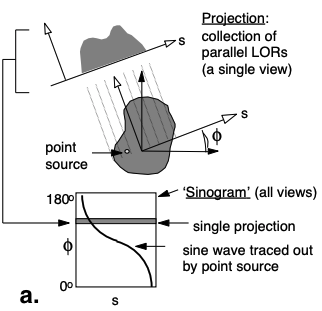
\includegraphics[width=\textwidth]{sinogram}
        \end{minipage}\hfill
        \begin{minipage}{0.55\textwidth}
        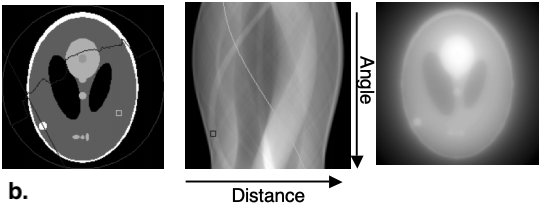
\includegraphics[width=\textwidth]{pet_recon.png}
        \caption{\textbf{a.} Sinogram data presentation. $\Phi$ and $s$ are the angle and distance of the point source from the center of the field of view. A single projection, $p(s,\Phi)$ fills one row in the sinogram. \textbf{b.} Example of PET reconstruction. Left: object image; middle: sinogram obtained via projection; right: reconstructed image from sinogram. \cite{adam2007intro}}
        % \label{fig:recon}
        \end{minipage}
        \label{fig:1}
        \vspace{-0.5cm}
    \end{figure}
    
    \noindent\textbf{Image reconstruction from sinogram:} As shown in Figure 1.b, image reconstruction is to reconstruct the objective image from the sinogram representing radiotracer distribution, which is a linear inverse problem. Assume the PET data contains no statistical noise, the imaging process could be formulated as a system of linear equations as $\mathbf{Hf=p}$, where $\mathbf{f}$ is a vector representing the object, $\mathbf{H}$ is the system matrix, and $\mathbf{p}$ is the sinogram ordered as a vector. The system matrix models the sensitivity at each point by modeling the probability of positron annihilated in this point and being detected as a coincidence event by the detector. However, the PET data has noises and uncertainties caused by multiple factors like scattering, low event count in photon detection, etc. So the formula is modified as $\mathbf{Hf+n=p}$, where $\mathbf{n}$ is the noise during the process, resulting in the ill-posedness problem. The goal to solve the inverse problem is to find the optimal matrix $\mathbf{H}$ to make reconstruction precise and robust.
    % An general way to improve the stability of the inverse problem is adding regularization terms that emphasize priori information \cite{tong2010petctreview}. 

    In practice, photon is attenuated when it fails to travel along a straight line caused by Compton scattering or other interactions, resulting in the largest degradation to PET data. Therefore, the projection data requires a bunch of pre-processing steps to deal with these impacts due to attenuation, scattering, and detector efficiency. 
    % in order to achieve quantitative imaging corresponding to the true strength of tissue activity at each point. 
    Conceptually, the measured projection $P$ are related to the true coincidence events T as $P=N(AT+S+R)$, where $A,R,S,N$ are attenuation, random, scatter, and normalization correction factors, respectively \cite{tong2010petctreview}.  

    \vspace{-0.5cm}
    \section{Classic Reconstruction Methods}
    \label{sec:method}
    The most commonly used PET reconstruction algorithms can be divided into 2 main categories: analytical reconstruction and iterative reconstruction. \\
    \textbf{Analytic image reconstruction:} This method assumes PET data is noise-free and attempts to find the system matrix directly. 
    % One way is the apply direct Fourier methods. They perform 1D Fourier transform (FT) of each single project in the sinogram, interpolate and sum the results in 2D Fourier domain, and then obtain the image by inverse 2D Fourier transform. However, the reconstruction quality is highly affected by interpolation errors. 
    The most common method is filtered backprojection (FBP). Its principle is backprojection, the reverse of data acquisition, that projects the counts from a detector pair into an image array along LOR. A linear superposition of backprojections could be obtained by repeating this process for all detector pairs. In detail, for each projection angle, 1) take 1D FT of the projection; 2) filter with ramp filter, e.g. Hann filters or Shepp-Logan filters; 3) take inverse FT to get the filtered projection; 4) backproject the filter project to obtain the image. The Analytic image reconstruction method is simple and computing efficient, but the reconstruction accuracy is limited for 2 major reasons. First, it fails to model the degrading factors such as intercrystal scatter, positron range, and noncollinearity. Second, it doesn't consider stochastic uncertainties in photon detection. Therefore, the analytic image reconstruction methods are seldom used in most application cases.\\
    \textbf{Iterative image reconstruction:} The algorithm's basic concept is to estimate the image progressively towards a better solution by modeling the statistical noise of PET data and physical effects of the imaging model. First, make an initial estimate of the objective distribution. Then calculate the estimated projection by forward projecting this initial estimate. Adjust the initial estimate by comparing the estimated and measured projection. Finally, repeat the previous two steps until the estimate reaches the desired solution. There are two key components required for all iterative methods: a criterion to define the 'better' image and an algorithm to determine how to update the image estimate at each iteration. Numerous studies have been performed in optimizing their designs. The most representative methods are Maximum-likelihood estimation (MLEM) and its variant Ordered subsets estimate (OSEM) \cite{tong2010petctreview}.\\
    \textbf{MLEM:} It's a standard statistical estimation method to maximize the likelihood function that most-likely leads to the measured data. MLEM adopts ML as the optimization criterion and EM algorithm to find the optima. For image reconstruction with Poisson likelihood, the MLEM could be formulated as the iterative equation: $f_j^{n+1}=(f_j^n/\sum_iH_{ij})\sum_iH_{ij}(p_i/\sum_jH_{ij}f_j^n)$, where $f_j^n$ is the image estimate of $i$th pixel at $k$th iteration, $p_j$ is the $j$th line-integral measured data, and $H$ is the system matrix. The summation over index $j$ is forward projector, and the summation over index $i$ is the backprojector. The flow of the algorithm is as described previously. This strategy serves as the foundation for other iterative methods. Although MLEM could converge consistently, it suffers very noisy reconstructed estimate due to ill-conditioning problem and slow convergence which need more computation source and time. Solutions for the noisy issue include early-stop strategy and applying smoothing filters.\cite{tong2010petctreview}\\
    \textbf{OSEM:} To address the issue of slow convergence, OSEM is proposed by partitioning the projection data into $B$ mutually exclusive subsets and using only one subset $S_b$ for each update. Previous update equation is modified as $f_j^{(n,b)}=(f_j^{(n,b-1)}/\sum_{i\in S_b}H_{ij})\sum_{i\in S_b}H_{ij}(p_i/\sum_jH_{ij}f_j^{n,b-1})$, where $b$ is the index for each subset. The number of subsets determines the degree of acceleration since each pass of the entire data has $B$ times number of updates. However, OSEM still faces the issue of the increased noise level. Another problem is no guaranteed convergence to ML\cite{portnow2013history}.
    % Of course, there are numerous other iterative methods proposed except for the MLEM and its variant OSEM. For instance, algebraic reconstruction techniques (ART) which use block-iterative method, and maximum a posteriori (MAP) reconstruction which maximizes the posterior probability density by introducing priori knowledge. 
    
    \vspace{-0.5cm}
    \section{Future Directions and Challenges}
    \label{sec:future}
    Since the last decades, reconstruction algorithms have achieved significant advances in multiple aspects aiming to reduce the noise level and obtain accurate image estimation, though there are still a bunch of problems that need to be solved. We choose several important aspects to discuss. 
    
    \noindent\textbf{3D reconstruction:} Unlike 2D imaging mode that collects data only from direct and cross planes, the 3D scanner collects data from all oblique planes. The fully 3D PET data is characterized by data redundancy and spatially-varying detector response. The observed intensity of a point source varies depending on its position in the scanner's field of view, making reconstruction more complicated. Similarly, the 2D analytical reconstruction and iterative image reconstruction methods could be extended to 3D by representing the object with voxels rather than 2D pixels. 
    % Besides, an intuitive solution is to convert 3D data to decoupled sets of 2D data and then apply 2D reconstruction. This strategy is rebinning methods, including single-slice rebinning and Fourier rebinning. 
    Compared to 2D reconstruction, the major challenge for 3D reconstruction methods is the rapidly increasing computation cost\cite{tong2010petctreview}. 

    \noindent\textbf{Time-of-Flight (TOF) imaging:} TOF imaging localizes the annihilation events along the LOR by measuring the arrival time difference of the two annihilation photons in the scanner. This technique requires a modern PET system with extremely high time resolution (~3ns). Although reconstruction is still needed for exact localization, this technique benefits the image quality especially signal-to-noise ratio. TOF-KEM reconstruction algorithm was proposed by Wang et al. to accommodate TOF data\cite{wang2021tof}. 

    \noindent\textbf{Combination of PET with CT or MRI:} PET imaging has relatively low resolution compared with CT and MRI. Additional anatomical information provided by these imaging modalities could guide imaging reconstruction and noised regularization. Maximum a posteriori (MAP) reconstruction algorithm which maximizes the posterior probability density by introducing priori knowledge is proposed to utilize multi-modality data. However, anatomical information from CT/MRI imaging needs segmentation with boundaries in advance, posing another challenge in CT/MRI imaging analysis\cite{tong2010petctreview}.

    \noindent\textbf{Potential of deep learning (DL) methods:} Currently, DL techniques have achieved widespread impacts on many computer vision tasks, including image classification, object detection, image generation, and inverse problems. Due to powerful data approximation abilities, they could learn the reconstruction operator that maps measurement data domain to imaging domain directly without much priori knowledge. DL based methods are also exploited in PET reconstruction. It mainly employs DL as 1) end-to-end mapping for direct reconstruction; 2) synthesis regularization for integrating sophisticated denoiser during reconstruction; 3) analysis regularization like conventional priori function to introduce additional knowledge; 4) preprocessing and post-processing for conventional algorithms. Particularly, large amounts of effort have been devoted to designing a good network architecture based on principles of linear direct mapping, convolution direct mapping, convolution with nonlinearity, deep networks, convolutional neural networks, and generative adversarial networks. The major challenge also lies in the high computation time and cost\cite{aj2020dl}.  
\vspace{-0.5cm}
{\small
\bibliographystyle{abbrv}
\bibliography{pet.bib}
}
\end{document}

